\documentclass[8pt,]{article}
\usepackage{lmodern}
\usepackage{amssymb,amsmath}
\usepackage{ifxetex,ifluatex}
\usepackage{fixltx2e} % provides \textsubscript
\ifnum 0\ifxetex 1\fi\ifluatex 1\fi=0 % if pdftex
  \usepackage[T1]{fontenc}
  \usepackage[utf8]{inputenc}
\else % if luatex or xelatex
  \ifxetex
    \usepackage{mathspec}
  \else
    \usepackage{fontspec}
  \fi
  \defaultfontfeatures{Ligatures=TeX,Scale=MatchLowercase}
\fi
% use upquote if available, for straight quotes in verbatim environments
\IfFileExists{upquote.sty}{\usepackage{upquote}}{}
% use microtype if available
\IfFileExists{microtype.sty}{%
\usepackage{microtype}
\UseMicrotypeSet[protrusion]{basicmath} % disable protrusion for tt fonts
}{}
\usepackage[left=1.5cm,right=1cm,top=2cm,bottom=2.2cm]{geometry}
\usepackage{hyperref}
\hypersetup{unicode=true,
            pdftitle={Paraguay},
            pdfauthor={The state of inequality in human capital},
            pdfborder={0 0 0},
            breaklinks=true}
\urlstyle{same}  % don't use monospace font for urls
\usepackage{graphicx,grffile}
\makeatletter
\def\maxwidth{\ifdim\Gin@nat@width>\linewidth\linewidth\else\Gin@nat@width\fi}
\def\maxheight{\ifdim\Gin@nat@height>\textheight\textheight\else\Gin@nat@height\fi}
\makeatother
% Scale images if necessary, so that they will not overflow the page
% margins by default, and it is still possible to overwrite the defaults
% using explicit options in \includegraphics[width, height, ...]{}
\setkeys{Gin}{width=\maxwidth,height=\maxheight,keepaspectratio}
\IfFileExists{parskip.sty}{%
\usepackage{parskip}
}{% else
\setlength{\parindent}{0pt}
\setlength{\parskip}{6pt plus 2pt minus 1pt}
}
\setlength{\emergencystretch}{3em}  % prevent overfull lines
\providecommand{\tightlist}{%
  \setlength{\itemsep}{0pt}\setlength{\parskip}{0pt}}
\setcounter{secnumdepth}{0}
% Redefines (sub)paragraphs to behave more like sections
\ifx\paragraph\undefined\else
\let\oldparagraph\paragraph
\renewcommand{\paragraph}[1]{\oldparagraph{#1}\mbox{}}
\fi
\ifx\subparagraph\undefined\else
\let\oldsubparagraph\subparagraph
\renewcommand{\subparagraph}[1]{\oldsubparagraph{#1}\mbox{}}
\fi

%%% Use protect on footnotes to avoid problems with footnotes in titles
\let\rmarkdownfootnote\footnote%
\def\footnote{\protect\rmarkdownfootnote}

%%% Change title format to be more compact
\usepackage{titling}

% Create subtitle command for use in maketitle
\providecommand{\subtitle}[1]{
  \posttitle{
    \begin{center}\large#1\end{center}
    }
}

\setlength{\droptitle}{-2em}

  \title{Paraguay}
    \pretitle{\vspace{\droptitle}\centering\huge}
  \posttitle{\par}
    \author{The state of inequality in human capital}
    \preauthor{\centering\large\emph}
  \postauthor{\par}
    \date{}
    \predate{}\postdate{}
  
\usepackage{fancyhdr}

\pagestyle{fancy}

\usepackage{graphicx} \usepackage{eurosym} \usepackage{booktabs,xcolor}

\rhead{October 2019} \rfoot{}
\lfoot{
\includegraphics[width=19.5cm]{static/footerpdf.pdf}}
\fancypagestyle{plain}{\pagestyle{fancy}} \pagenumbering{gobble}

\usepackage[pagecolor={white}, nopagecolor={none}]{pagecolor} \usepackage{librebaskerville} \usepackage[fontsize=8pt]{scrextend} \usepackage{float}

\restylefloat{table}

\usepackage{xcolor} \usepackage{multicol} \newcommand{\hideFromPandoc}[1]{#1}

 \let\Begin\begin \let\End\end 

\usepackage{caption}

\captionsetup{skip=0pt}

\begin{document}
\maketitle

\definecolor{bondiblue}{rgb}{0.0, 0.58, 0.71}
\newcommand\boldblue[1]{\textcolor{bondiblue}{\textbf{#1}}}

The launch of the Human Capital Index (HCI) in October 2018 underscored
a huge gap in human capital outcomes across regions and income groups.
As a measure of the relative productivity of the next generation of
workers, the HCI shows the effectiveness of current investments and the
readiness of a country to be competitive in an increasingly complex
world with constantly changing nature of work. Equally important as a
country's average distance from the frontier is how different
socio-economic groups fare in terms of their relative future
productivity. In a world where rising inequality is a critical policy
issue, narrowing differences in human capital outcomes across
socio-economic groups could be a way to facilitate economic mobility.

This country profile presents the data on disaggregation of HCI and its
components (\textbf{child survival, expected years of school, harmonized
test scores and non-stunted rate}) by socio-economic status. The
objective of this exercise is to look at differences within countries
and is not meant to be comparable with the cross-country HCI values
published earlier. While the exercise employs a similar methodology, it
is different in that it excludes adult survival rate and is based on
household survey based enrolment rates of children ages 6-17. The
disaggregation is available for 51 countries. Given that human capital
outcomes may not be uniquely increasing/decreasing across socio-economic
groups, this country profile provides a comparison of the richest and
poorest 20 percent of households.

\begin {multicols}{2}

\hypertarget{section}{%
\subsubsection{\texorpdfstring{\textcolor{bondiblue}{\textbf{H\small{OW DOES THE POOREST 20 PERCENT FARE COMPARED TO THE RICHEST?}}}}{}}\label{section}}

\begin{itemize}
\item
  \textbf{Human Capital Index (HCI).} In Paraguay, the productivity as a
  future worker of a child born today in the richest 20 percent of
  households is \textbf{71 percent} while it is \textbf{56 percent} for
  a child born in the poorest 20 percent, a gap of \textbf{16}
  percentage points. This gap is about the same as the typical gap
  across the 51 countries (15 percentage points).
\item
  \textbf{Probability of Survival to Age 5.} In Paraguay, the
  probability of survival of a child born today in the richest 20
  percent of households is \textbf{100 percent} while it is \textbf{97
  percent} for a child born in the poorest 20 percent, a gap of
  \textbf{2} percentage points. This gap is slightly smaller than the
  typical gap across the 51 countries (4percentage points).
\item
  \textbf{Expected Years of School.} In Paraguay, a child in the richest
  20 percent of households who starts school at age 6 can expect to
  complete \textbf{11.4 years} of school by her 18th birthday while a
  child from the poorest 20 percent can expect to complete \textbf{9.8
  years} of school, a gap of \textbf{1.7 years} of school. This gap is
  smaller than the typical gap across the 51 countries (2.4years).
\item
  \textbf{Harmonized Test Scores.} Students from the richest 20 percent
  of households in Paraguay score \textbf{429} while those from the
  poorest 20 percent score \textbf{359}, a gap of \textbf{69 points}.
  This gap is larger than the typical gap across the 51 countries
  (56points).
\item
  \textbf{Healthy Growth (Not Stunted Rate).} In Paraguay, the
  percentage of children in the top 20 percent of households who are not
  stunted is \textbf{99 percent} while it is \textbf{87 percent} among
  the poorest 20 percent, a gap of \textbf{12} percentage points. This
  gap is smaller than the typical gap across the 51 countries (19
  percentage points).
\end{itemize}

\begin{flushright}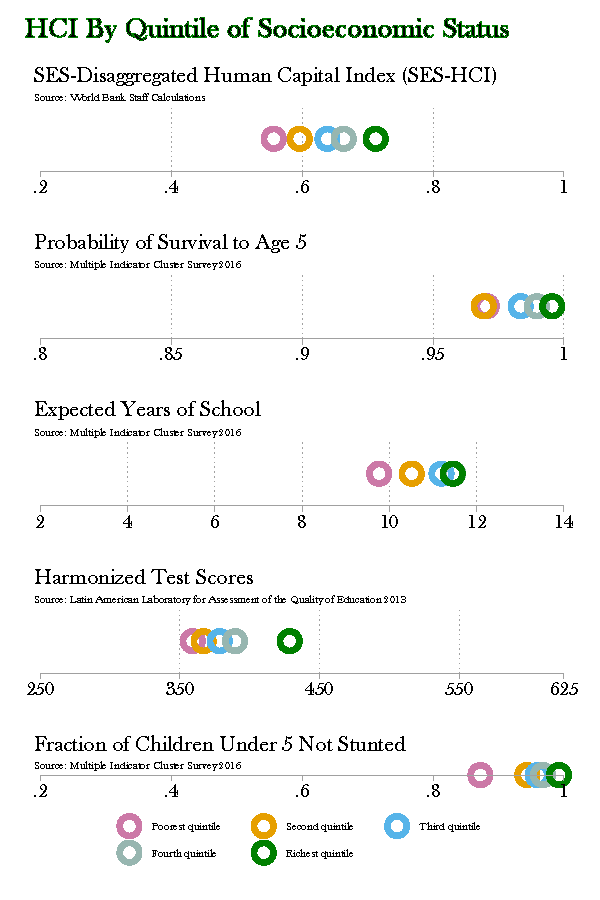
\includegraphics[width=1\linewidth]{charts/ses_PRY} \end{flushright}

\noindent

\rule{9cm}{0.4pt}

The Human Capital Project is a global effort to accelerate the amount
and quality of investments in people. ~

For more information on the Human Capital Project, please visit
\textbf{\href{https://www.worldbank.org/humancapitalproject}{www.worldbank.org/humancapitalproject}}

\begin{table}[H]
\begin{tabular}{ll}

\includegraphics[width=0.5cm]{static/twitter.png} & \#\textbf{invest}inPeople   \\
\end{tabular}
\end{table}

\end {multicols}


\end{document}
